\documentclass[a4paper,12pt,twoside,final,spanish]{article}
%titlepage: pone el título en una página aparte
%twocolumn
\usepackage{babel} %Para el lenguaje [spanish]
\usepackage[utf8]{inputenc} %Para reconocer todos los símbolos
\usepackage[T1]{fontenc}
\usepackage{textcomp}
\usepackage{amsmath}
\usepackage{amsfonts}
\usepackage{amssymb}
\usepackage[margin=1.5cm]{geometry} %Márgenes
\usepackage[T1]{fontenc}
\usepackage{graphicx}
\usepackage{enumerate}
\usepackage{hyperref}
%\pagestyle{headings}

%---
\usepackage{geometry} %Algo de las líneas del pie y encabezados
\geometry{text={7in,9.5in},headheight=15pt}
%\textwidth = 7 in
%\textheight = 9.5 in
%\oddsidemargin = -0.25 in
%\evensidemargin = 0.0 in
%\topmargin = -0.25 in
%\headheight = 0.0 in
%\headsep = 0.0 in
\setlength{\parskip}{0.1in}
\setlength{\parindent}{0.0in}
%---
\usepackage{fancyhdr} %Para usar encabezados y pies personalizados
	\pagestyle{fancy}
	\fancyhf{}
	\fancyhead[LE,RO]{Tecnologías para la Web Semántica} 
	\fancyhead[RE,LO]{Arquitectura}
	\fancyfoot[RE,LO]{Darién Julián Ramírez}
	\fancyfoot[LE,RO]{\thepage}
	\renewcommand{\footrulewidth}{1pt}
%---
\usepackage{listings} %Para escribir códigos
\lstset{language=XML,
	basicstyle=\footnotesize,
	numbers=left,
 	stepnumber=1,
	numbersep=8pt,
	showspaces=false,               % show spaces adding particular underscores
  	showstringspaces=false,         % underline spaces within strings
  	frame=lines,                   % adds a frame around the code
	tabsize=4,                      
  	captionpos=b,                   % sets the caption-position to bottom
  	breaklines=true,                % sets automatic line breaking
}
%---

\title{\Huge Tecnologías para la Web Semántica\\
Trabajo Práctico Nº6\\
OWL}
\author{Darién Julián Ramírez}
\date{\vspace{-5ex}}

\begin{document}

\maketitle %Crea la página de título

\section*{Ejercicio 1}

Analice el código OWL de la ontología \textit{An African Wildlife Ontology} (A 
Semantic Web Primer, Antoniou, 2002).

\begin{enumerate}[a.]
\item Identifique los componentes con su respectivo vocabulario (rdf, rdfs ,owl)
	\begin{itemize}
	\item Clases y jerarquía.
	\begin{quote}
	\begin{itemize}
		\item Nivel 1: Animal, Plant.
		\item Nivel 2: Carnivore, Herbivore, Tree, Tasty plant.
		\item Nivel 3: Lion, Girafe, Branch.
		\item Nivel 4: Leaf.
	\end{itemize}
	\end{quote}
	\item Relaciones.
	
	eats, eaten-by.
	
	\item Propiedades.
	
	TransitiveProperty, ObjectProperty.
	
	\item Restricciones.
	
	allValuesFrom, someValuesFrom.
	
	\end{itemize}
	
\item Realice el modelo correspondiente.

\begin{quote}
\begin{center}

\includegraphics[width=0.9\linewidth,keepaspectratio]{1.jpg}
\end{center}
\end{quote}
	
\end{enumerate}

\begin{lstlisting}
<rdf:RDF
	xmlns:rdf="http://www.w3.org/1999/02/22-rdf-syntaxns#"
	xmlns:rdfs="http://www.w3.org/2000/01/rdf-schema#"
	xmlns:owl ="http://www.w3.org/2002/07/owl#"
	xmlns="http://www.mydomain.org/african">
	
	<owl:Ontology rdf:about="">
		<owl:VersionInfo>
			My example version 1.2, 17 October 2002
		</owl:VersionInfo>
	</owl:Ontology>
	
	<owl:Class rdf:ID="animal">
		<rdfs:comment>Animals form a class</rdfs:comment>
	</owl:Class>
	
	<owl:Class rdf:ID="plant">
		<rdfs:comment>
			Plants form a class disjoint from animals
		</rdfs:comment>
		<owl:disjointWith="#animal"/>
	</owl:Class>
	
	<owl:Class rdf:ID="tree">
		<rdfs:comment>
			Trees are a type of plants
		</rdfs:comment>
		<rdfs:subClassOf rdf:resource="#plant"/>
	</owl:Class>
	
	<owl:Class rdf:ID="branch">
		<rdfs:comment>
			Branches are parts of trees
		</rdfs:comment>
		<rdfs:subClassOf>
			<owl:Restriction>
				<owl:onProperty rdf:resource="#is-part-of"/>
				<owl:allValuesFrom rdf:resource="#tree"/>
			</owl:Restriction>
		</rdfs:subClassOf>
	</owl:Class>
	
	<owl:Class rdf:ID="leaf">
		<rdfs:comment>
			Leaves are parts of branches
		</rdfs:comment>
		<rdfs:subClassOf>
			<owl:Restriction>
				<owl:onProperty rdf:resource="#is-part-of"/>
				<owl:allValuesFrom rdf:resource="#branch"/>
			</owl:Restriction>
		</rdfs:subClassOf>
	</owl:Class>
	
	<owl:Class rdf:ID="herbivore">
		Web Ontology Language: OWL 19
		<rdfs:comment>
			Herbivores are exactly those animals that eat only plants, or parts of plants
		</rdfs:comment>
		<owl:intersectionOf rdf:parsetype="Collection">
			<owl:Class rdf:about="#animal"/>
			<owl:Restriction>
				<owl:onProperty rdf:resource="#eats"/>
				<owl:allValuesFrom>
					<owl:unionOf rdf:parsetype="Collection">
						<owl:Class rdf:about="#plant"/>
						<owl:Restriction>
							<owl:onProperty rdf:resource="#is-part-of"/>
							<owl:allValuesFrom rdf:resource="#plant"/>
						</owl:Restriction>
					</owl:unionOf>
				</owl:allValuesFrom>
			</owl:Restriction>
		</owl:intersectionOf>
	</owl:Class>
	
	<owl:Class rdf:ID="carnivore">
		<rdfs:comment>
			Carnivores are exactly those animals that eat also animals
		</rdfs:comment>
		<owl:intersectionOf rdf:parsetype="Collection">
			<owl:Class rdf:about="#animal"/>
			<owl:Restriction>
				<owl:onProperty rdf:resource="#eats"/>
				<owl:someValuesFrom rdf:resource="#animal"/>
			</owl:Restriction>
		</owl:intersectionOf>
	</owl:Class>
	
	<owl:Class rdf:ID="giraffe">
		<rdfs:comment>
			Giraffes are herbivores, and they eat only leaves
		</rdfs:comment>
		<rdfs:subClassOf rdf:type="#herbivore"/>
		<rdfs:subClassOf>
			<owl:Restriction>
				<owl:onProperty rdf:resource="#eats"/>
				<owl:allValuesFrom rdf:resource="#leaf"/>
			</owl:Restriction>
		</rdfs:subClassOf>
	</owl:Class>
	
	<owl:Class rdf:ID="lion">
		<rdfs:comment>
			Lions are animals that eat only herbivores
		</rdfs:comment>
		<rdfs:subClassOf rdf:type="#carnivore"/>
			20 Grigoris Antoniou and Frank van Harmelen
		<rdfs:subClassOf>
			<owl:Restriction>
				<owl:onProperty rdf:resource="#eats"/>
				<owl:allValuesFrom rdf:resource="#herbivore"/>
			</owl:Restriction>
		</rdfs:subClassOf>
	</owl:Class>
	
	<owl:Class rdf:ID="tasty-plant">
		<rdfs:comment>
			Tasty plants are plants that are eaten both by herbivores and carnivores
		</rdfs:comment>
		<rdfs:subClassOf rdf:resource="#plant"/>
		<rdfs:subClassOf>
			<owl:Restriction>
				<owl:onProperty rdf:resource="#eaten-by"/>
				<owl:someValuesFrom>
					<owl:Class rdf:about="#herbivore"/>
				</owl:someValuesFrom>
			</owl:Restriction>
		</rdfs:subClassOf>
		<rdfs:subClassOf>
			<owl:Restriction>
				<owl:onProperty rdf:resource="#eaten-by"/>
				<owl:someValuesFrom>
					<owl:Class rdf:about="#carnivore"/>
				</owl:someValuesFrom>
			</owl:Restriction>
		</rdfs:subClassOf>
	</owl:Class>
	
	<owl:TransitiveProperty rdf:ID="is-part-of"/>
	<owl:ObjectProperty rdf:ID="eats">
		<rdfs:domain rdf:resource="#animal"/>
	</owl:ObjectProperty>
	<owl:ObjectProperty rdf:ID="eaten-by">
		<owl:inverseOf rdf:resource="#eats"/>
	</owl:ObjectProperty>
</rdf:RDF>
\end{lstlisting}

\section*{Ejercicio 2}

Analice el código OWL de la ontología:\\
\url{http://www.cs.man.ac.uk/~rector/Modules/CS646-2004/Labs/ThursdaySimple_University-01.owl}

\begin{enumerate}[a.]
\item Identifique los componentes:
	\begin{itemize}
	\item \textbf{Clases y jerarquía}
		
	Senior lecturer[OWL](Academic rank[RDFS]) \\
	Course[OWL](Teaching unit[RDFS] \\
	Academic staff[RDFS]) \\
	Long thin format[OWL](Module format[RDFS]) \\
	Short fat format[OWL] \\
	Las dos clases anteriores son disjuntas. \\
	White ethnicity[OWL](Ethnicity Value Type[RDFS]) \\
	Modules with exams[OWL] (Equivalente a intersección de module y exam.)\\
	Module[OWL] \\
	Exam[OWL] \\
	Functional roles[OWL] \\
	Module format[OWL](Pattern[RDFS]) \\
	female[OWL](Sex Value Type[RDFS]) (Disjunta de male)\\
	black woman professor [OWL] (Equivalente a la intersección de person, 					professor rank y black ethnicity) \\
	...
		
    \item \textbf{Relaciones }
    
    has part (Transitiva para la intersección de module y exam) \\
	has academic rank \\
	has sex\\
	hasSalaryRange\\
	attends\\
	isGivenBy\\
	RV property\\
	gives \\
    
	\item \textbf{Propiedades:}
	
	TransitiveProperty \\
	FunctionalProperty \\
	ObjectProperty \\
		
	\item \textbf{Restricciones}
	
	someValuesFrom \\
		
	\end{itemize}

\item Realice el modelo correspondiente.

\begin{figure}[htbp]
\centerline{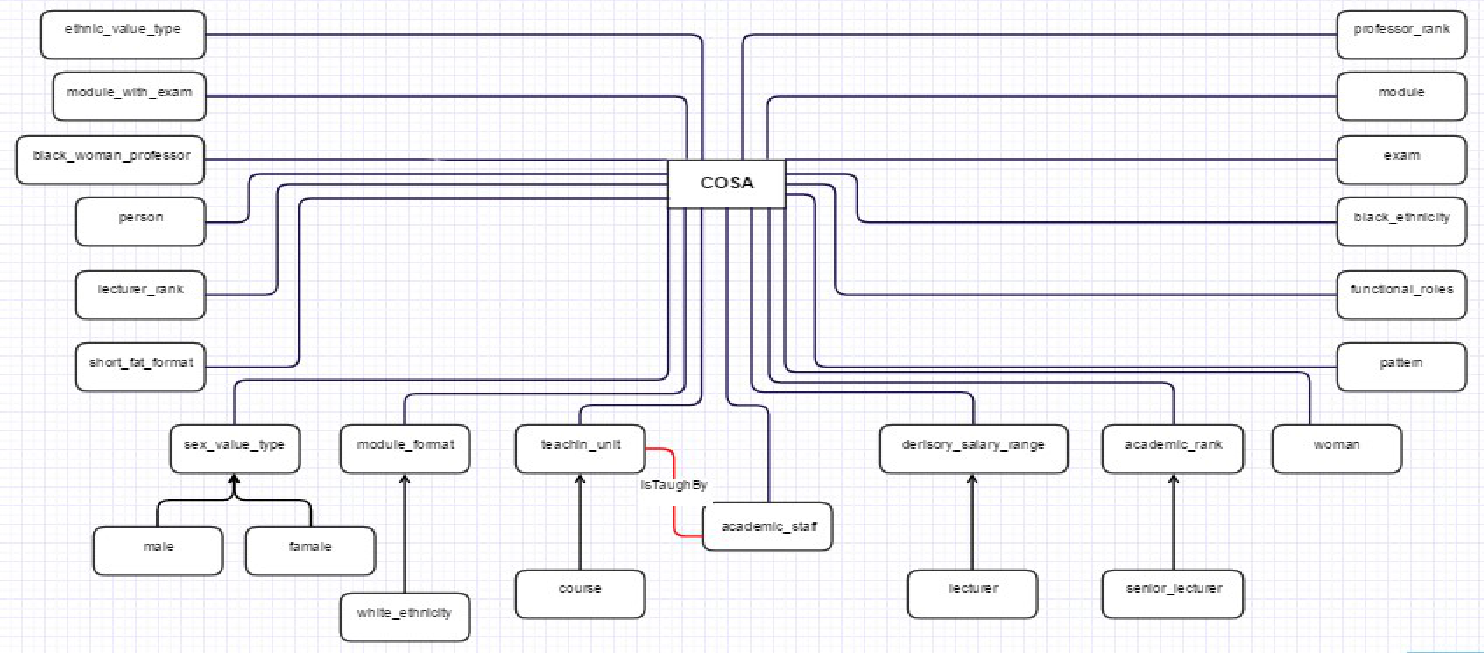
\includegraphics[width=\linewidth]{ej2}}
\caption{Modelo del ejercicio 2.}
\label{fig:ej2}
\end{figure}

\end{enumerate}

\end{document}